%!TEX root = ../report.tex
\section{Echo-SLAM}

\subsection{Sine Sweep Generation}

\subsection{RIR recording}

\subsection{Analysis}

%\begin{lstlisting}[caption=Listing]
%\end{lstlisting}

%\begin{figure}[H]
%	\centering
%	\begin{subfigure}[b]{0.49\linewidth}
%		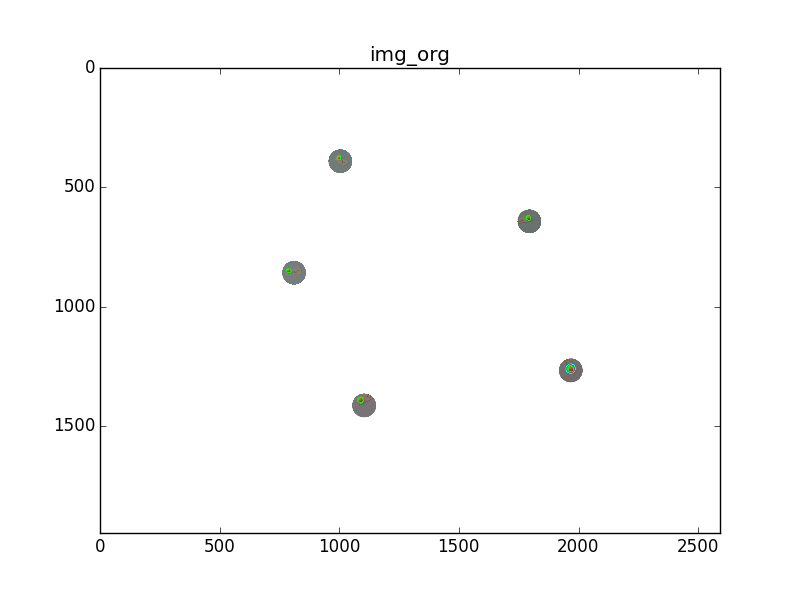
\includegraphics[width=\linewidth]{../files/img_org139.png}
%		\caption{Regions of interest chosen by user and extracted colors}
%		\label{feat_step0}
%	\end{subfigure}
%	\begin{subfigure}[b]{0.49\linewidth}
%		\includegraphics[width=\linewidth]{../files/img_h139.png}
%		\caption{\textit{Hue} representation of original image}
%		\label{feat_step1}
%	\end{subfigure}
%	\begin{subfigure}[b]{0.49\linewidth}
%		\includegraphics[width=\linewidth]{../files/img_s139.png}
%		\caption{\textit{Saturation} representation of original image}
%		\label{feat_step2}
%	\end{subfigure}
%	\begin{subfigure}[b]{0.49\linewidth}
%		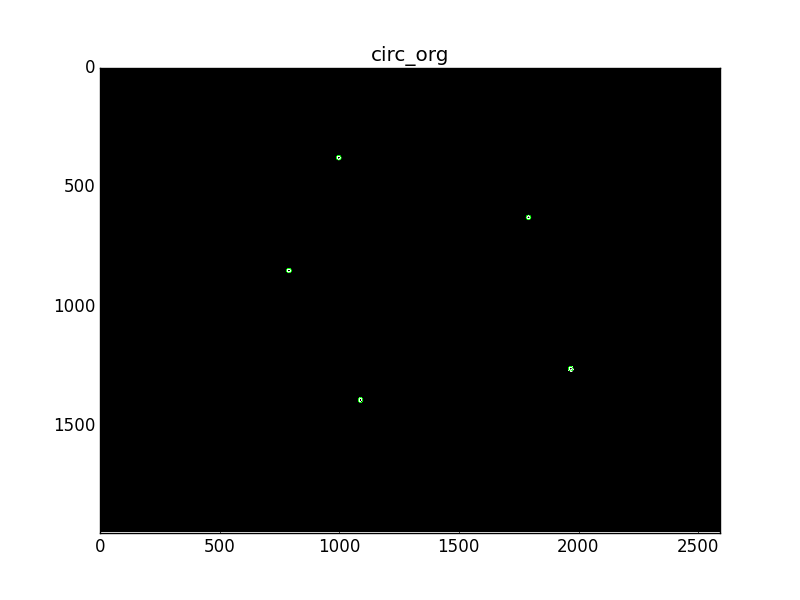
\includegraphics[width=\linewidth]{../files/circ_org139.png}
%		\caption{Regions of interest chosen by user and extracted colors}
%		\label{feat_step3}
%	\end{subfigure}
%	
%	
%	\begin{subfigure}[b]{0.49\linewidth}
%		\includegraphics[width=\linewidth]{../files/zdot_RefTrackNL.png}
%	\end{subfigure}
%	\begin{subfigure}[b]{0.49\linewidth}
%		\includegraphics[width=\linewidth]{../files/speeds_RefTrackNL.png}
%	\end{subfigure}
%	\begin{subfigure}[b]{0.49\linewidth}
%		\includegraphics[width=\linewidth]{../files/xyz_RefTrackNL.png}
%	\end{subfigure}
%	\caption{Procedure for feature extraction} 
%	\label{features}
%\end{figure}
